\documentclass{sigchi}

% Use this section to set the ACM copyright statement (e.g. for
% preprints).  Consult the conference website for the camera-ready
% copyright statement.

% Copyright
%\CopyrightYear{2018}
%\setcopyright{acmcopyright}
%\setcopyright{acmlicensed}
%\setcopyright{rightsretained}
%\setcopyright{usgov}
%\setcopyright{usgovmixed}
%\setcopyright{cagov}
%\setcopyright{cagovmixed}
% DOI
% ISBN
%Conference
%Price

% Use this command to override the default ACM copyright statement
% (e.g. for preprints).  Consult the conference website for the
% camera-ready copyright statement.

%% HOW TO OVERRIDE THE DEFAULT COPYRIGHT STRIP --
%% Please note you need to make sure the copy for your specific
%% license is used here!
\toappear{2018 Hochschule München}

% Arabic page numbers for submission.  Remove this line to eliminate
% page numbers for the camera ready copy
% \pagenumbering{arabic}

\RequirePackage{luatex85}

% Load basic packages
\usepackage{balance}       % to better equalize the last page
\usepackage{graphics}      % for EPS, load graphicx instead 
%\usepackage[T1]{fontenc}   % for umlauts and other diaeresis
\usepackage{fontspec}
\usepackage{txfonts}
\usepackage{mathptmx}
\usepackage[pdflang={de-DE}]{hyperref}
\usepackage{color}
\usepackage{booktabs}
\usepackage{textcomp}

% Some optional stuff you might like/need.
\usepackage{microtype}        % Improved Tracking and Kerning
% \usepackage[all]{hypcap}    % Fixes bug in hyperref caption linking
\usepackage{ccicons}          % Cite your images correctly!
\usepackage[utf8]{inputenc} % for a UTF8 editor only
\usepackage[ngerman]{babel}

\usepackage{todonotes}

% Paper metadata (use plain text, for PDF inclusion and later
% re-using, if desired).  Use \emtpyauthor when submitting for review
% so you remain anonymous.
\def\plaintitle{Secure Social Network - Parallel World}
\def\plainauthor{Dimitrie Diez, Daniel Graf, Ludwig Wagner}
\def\emptyauthor{Dimitrie Diez, Daniel Graf, Ludwig Wagner}
\def\plainkeywords{Authentifizierung; Authentifizierungsmechanismus; Authentifizierungskonzept; Fake-Profil; Parallel World; Always Login; Fake-Welt; Soziales Netzwerk; Sicherheitskonzept}

\def\plaingeneralterms{Documentation, Standardization}

% llt: Define a global style for URLs, rather that the default one
\makeatletter
\def\url@leostyle{%
  \@ifundefined{selectfont}{
    \def\UrlFont{\sf}
  }{
    \def\UrlFont{\small\bf\ttfamily}
  }}
\makeatother
\urlstyle{leo}

% To make various LaTeX processors do the right thing with page size.
\def\pprw{8.5in}
\def\pprh{11in}
\special{papersize=\pprw,\pprh}
\setlength{\paperwidth}{\pprw}
\setlength{\paperheight}{\pprh}
\setlength{\pdfpagewidth}{\pprw}
\setlength{\pdfpageheight}{\pprh}

% Make sure hyperref comes last of your loaded packages, to give it a
% fighting chance of not being over-written, since its job is to
% redefine many LaTeX commands.
\definecolor{linkColor}{RGB}{6,125,233}
\hypersetup{%
  pdftitle={\plaintitle},
% Use \plainauthor for final version.
%  pdfauthor={\plainauthor},
  pdfauthor={\emptyauthor},
  pdfdisplaydoctitle=true, % For Accessibility
  bookmarksnumbered,
  pdfstartview={FitH},
  colorlinks,
  citecolor=black,
  filecolor=black,
  linkcolor=black,
  urlcolor=linkColor,
  breaklinks=true,
  hypertexnames=false
}

% create a shortcut to typeset table headings
% \newcommand\tabhead[1]{\small\textbf{#1}}

% End of preamble. Here it comes the document.
\begin{document}

\title{\plaintitle}

\numberofauthors{3}
\author{%
  \alignauthor{Daniel Graf\\
    \affaddr{Hochschule München}\\
    \affaddr{München}\\
    \email{graf12@hm.edu}}\\
  \alignauthor{Ludwig Wagner\\
    \affaddr{Hochschule München}\\
    \affaddr{München}\\
    \email{wagner43@hm.edu}}\\
  \alignauthor{Dimitrie Diez\\
    \affaddr{Hochschule München}\\
    \affaddr{München}\\
    \email{diez@hm.edu}}\\
}

\maketitle

\begin{abstract}
In der heutigen Zeit existieren zahlreiche unterschiedliche Authentifizierungsverfahren, die den Menschen vertraut sind. Der Mensch nutzt heute verschiedene Plattformen und Devices um Informationen aufzubewahren oder mit anderen Personen zu teilen. Der Zugang zu diesen Daten muss durch Authentifizierungsverfahren bestmöglich geschützt werden. Die am häufigsten verwendete Methode ist E-Mail Adresse und Passwort.\cite{passwordsCommon}

Bei zahlreichen Onlineplattformen, wie beispielsweise Yahoo, SchülerVZ oder Sony wurden Millionen Kundendatensätze gestohlen und im Darknet veröffentlicht.\cite{darknetYahoo}

In diesen Fällen fehlen Angreifern lediglich die Passwörter um in die Accounts zu gelangen. Diese versuchen Angreifer häufig durch Brute-Force Angriffe zu ermitteln.\cite{bruteForce}

Der Erfolg dieser Methode basiert darauf, dass der Angreifer bei fehlerhaften Login Informationen informiert wird. Um dies zu verhindern wurde ein Konzept für einen Authentifizierungsvorgang entwickelt, bei dem der Angreifer genau diese Informationen nicht erhält. Das Konzept wurde für Soziale Netzwerke ausgelegt, ist jedoch vielseitig, beispielsweise auch für E-Mail Accounts, verwendbar. Bei einem fehlgeschlagenen Authentifizierungsvorgang wird ein erfolgreicher Login durch die Anzeige eines möglichst realen Fake-Kontos vorgetäuscht.

Um das Konzept zu bewerten und zu verfeinern, wurde eine Gruppenbefragung durchgeführt und mit Hilfe der gewonnenen Erkenntnisse ein Schema für Einzelbefragungen erarbeitet. Aus den anschließenden Einzelbefragungen ging hervor, welche Punkte bei der Umsetzung zu beachten sind, um eine gute Akzeptanz der Benutzer zu erreichen. Es hat sich ergeben, dass es wichtig ist, den Fokus auf Benutzerfreundlichkeit zu legen, um diese Akzeptanz zu erreichen.

Darauf basierend wurden für die Umsetzung des Konzepts verschiedene Handlungsempfehlungen erarbeitet und limitierende Faktoren aufgezeigt. Anschließend erfolgt eine Bewertung des Konzepts hinsichtlich Sicherheit, Umsetzbarkeit und Benutzbarkeit. 
\end{abstract}

%\category{K.6.5}{Management of Computing and Information Systems}{Security and Protection} 
%\category{K.4.2}{Computers and Society}{Social Issues}
%\keywords{\plainkeywords}

%%% BEGIN

\section{Einleitung}
In der Vergangenheit wurden häufig schwerwiegende Sicherheitslücken auf verschiedenen Online Plattformen für soziale Medien genutzt, um private Daten der Benutzer abzugreifen und die Accounts zur massiven Verbreitung von Werbung zu nutzen. Durch die steigende Aktivität der Hackerszene kam es in den letzten Jahren fortlaufend zu einem Anstieg der Cyberkriminalität. \cite{bkaInternertkrimi}

Trotz dieser Tatsachen machen sich nur wenige Benutzer Gedanken über den Schutz ihres Accounts. \cite{benutzerGedanken} Viele Benutzer sind gar nicht erst bereit, zusätzlichen Aufwand zu betreiben, um einen besseren Schutz der Benutzerkonten zu erreichen. Selbst wenn erweiterte Schutzmethoden wie z.B. Two-Factor-Authenfication zur Verfügung stehen, werden diese meist nur von wenigen Nutzern aktiv genutzt. \cite{benutzungTwoFactor} Der Nutzungskomfort eines einfachen Logins steht im Vordergrund. Dies zeigt, dass es vor allem in der Verantwortung der Betreiber von Plattformen liegt, neue Authentifizierungsverfahren zu entwickeln, die ohne störenden Mehraufwand einen besseren Schutz gewährleisten.

Der größte Angriffspunkt eines regulären Logins besteht darin, dass der Angreifer darüber informiert wird, wenn der Login fehlgeschlagen ist. So lässt sich der Login mit verschiedenen Passwörtern wiederholen, bis das richtige Passwort erraten wurde. Durch den von den Nutzern geschätzten Komfort, werden meist einfache Passwörter gewählt, die durch einen Brute-Force Angriff schnell erraten werden können. \cite{benutzerGedanken}

Um nun die Sicherheit von sozialen Netzwerken zu erhöhen, ohne den Nutzer mit einem Mehraufwand zu belasten, muss genau an dieser Stelle ein neues Konzept erarbeitet werden.


\section{Sachverwandte Arbeiten}
Das Thema wurde bereits in mehreren Arbeiten unterschiedlicher Autoren untersucht und behandelt. Viele Arbeiten zeigen dabei, dass die Sicherheit durch einen Login mit Benutzername und Passwort nicht ausreichend ist. \cite{passwordsAreDead} \cite{taneski2014password}

Infolge dessen wurde von ebenso vielen Autoren auf vielseitige Art und Weise untersucht, wie sich die Sicherheit verbessern lässt. Dabei wird der Fokus in den meisten Arbeiten auf alternative oder erweiterte Mechanismen zur Authentifizierung der Benutzer gelegt. Die Benutzerfreundlichkeit gerät dabei oft in den Hintergrund. \cite{karapanos2015sound} \cite{amin2017security} \cite{jarecki2018two}

Diese Arbeit setzt an einer anderen Stelle an und nimmt es sich zum Ziel, einen idealen Mittelweg zwischen minimalem Mehraufwand und maximaler Sicherheit zu erreichen. Die gewohnte Benutzerfreundlichkeit wird durch die Nutzung der gewohnten Login Mechanismen sichergestellt, während die Sicherheit durch Verwirrung möglicher Angreifer erzielt wird. 

\section{Beschreibung des Konzepts}
\label{Konzept}
Kernpunkt des Konzept ist die Erschaffung eines parallelen Fake-Netzwerkes. Dadurch soll verhindert werden, dass ein Angreifer in das Netzwerk gelangt oder Informationen über die Mitglieder des Netzwerkes gewinnen kann. Die Sicherheit wird somit durch Verwirrung erzeugt. Im folgenden wird der Aufbau des Netzwerkes anhand eines Login-Vorgangs beschrieben. \\
Auf der Startseite des Netzwerkes werden die Nutzer zunächst aufgefordert E-Mail Adresse und Passwort einzugeben, bevor sie zum zweiten Schritt der Authentifizierung gelangen. Hierfür muss jeder Nutzer bei der Registrierung eines, oder mehrere Authentifizierungsverfahren hinterlegen. Zur Auswahl stehen beispielsweise ein Code, welcher per SMS zugesandt wird, eine Push-Benachrichtigung am Mobiltelefon oder die Verwendung biometrischer Daten (z.B Fingerabdruck).\\
Unabhängig davon, ob E-Mail Adresse, Passwort, die Wahl des zusätzlichen Verfahrens oder die Durchführung des gewählten Verfahrens korrekt waren, gelangt der Nutzer in das Netzwerk. Doch nur im Falle eines vollständig korrekten Authentifizierungsvorgangs befindet sich der Nutzer in seinem Account im \glqq echten\grqq Netzwerk. Andernfalls gelangt der Nutzer in ein täuschend echt aussehendes Fake-Profil, welches nur vom Inhaber als solches enttarnt werden kann. Der Login Vorgang ist in Abbildung \ref{fig:Login} aufgeführt. 
\begin{figure}[htbp]
\centering
	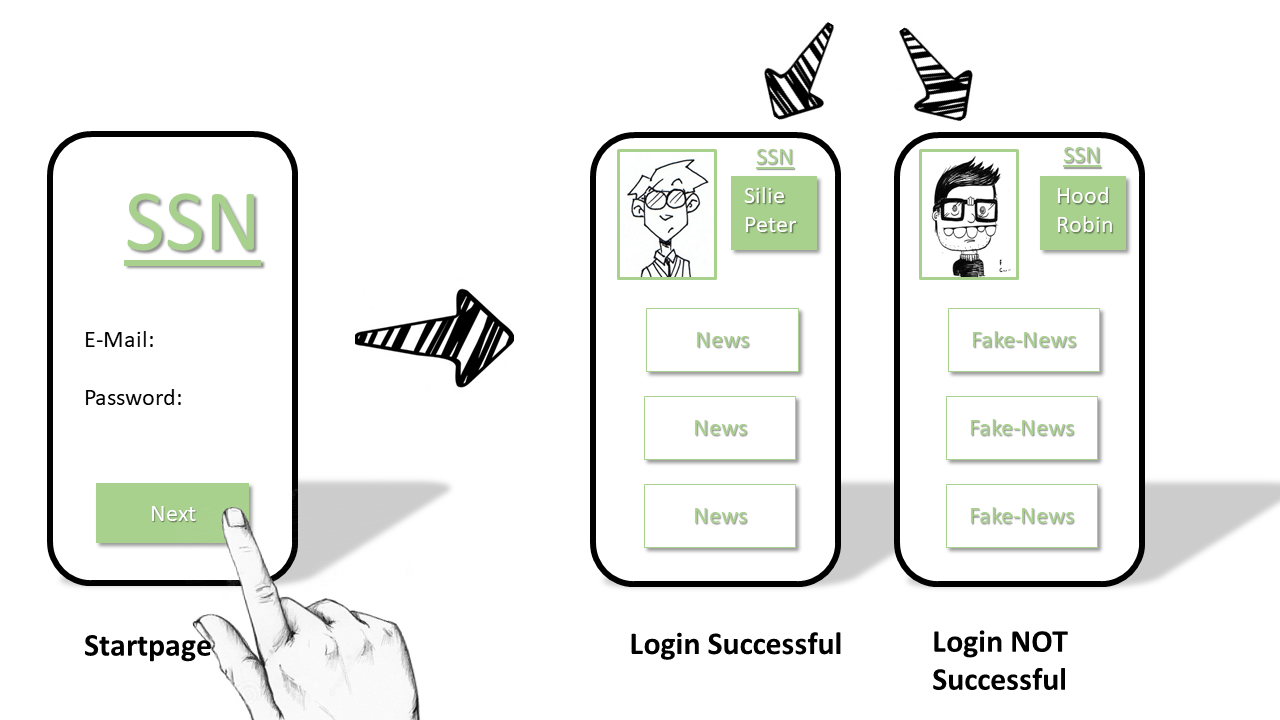
\includegraphics[width=0.8\columnwidth]{figures/Loginvorgang.png}
	\caption{Login Vorgang}
	\label{fig:Login}
\end{figure}
Der Angreifer erfährt dadurch weder ob seine eingegebenen Angaben korrekt waren bzw. welche nicht korrekt waren, noch kann er sich sicher sein, ob er im echten Netzwerk ist. Sämtliche, für ihn sichtbaren Informationen sind folglich nicht verifizierbar und daher nahezu wertlos. \\
Die größte Herausforderung bei der Umsetzung des Konzeptes stellt die Generierung des Fake-Netzwerkes dar. Hierfür wurden 4 unterschiedliche Umsetzungsvarianten definiert, welche im Folgenden beschrieben werden. \\
In der ersten Variante, muss jeder Nutzer bei der Registrierung neben seinem echten Profil auch ein Fake-Profil anlegen. Ob er hierbei korrekte oder falsche Angaben macht kann jeder Nutzer selbst entscheiden. Abbildung \ref{fig:Umsetzung1} zeigt ein Beispiel hierfür. 
\begin{figure}[htbp]
\centering
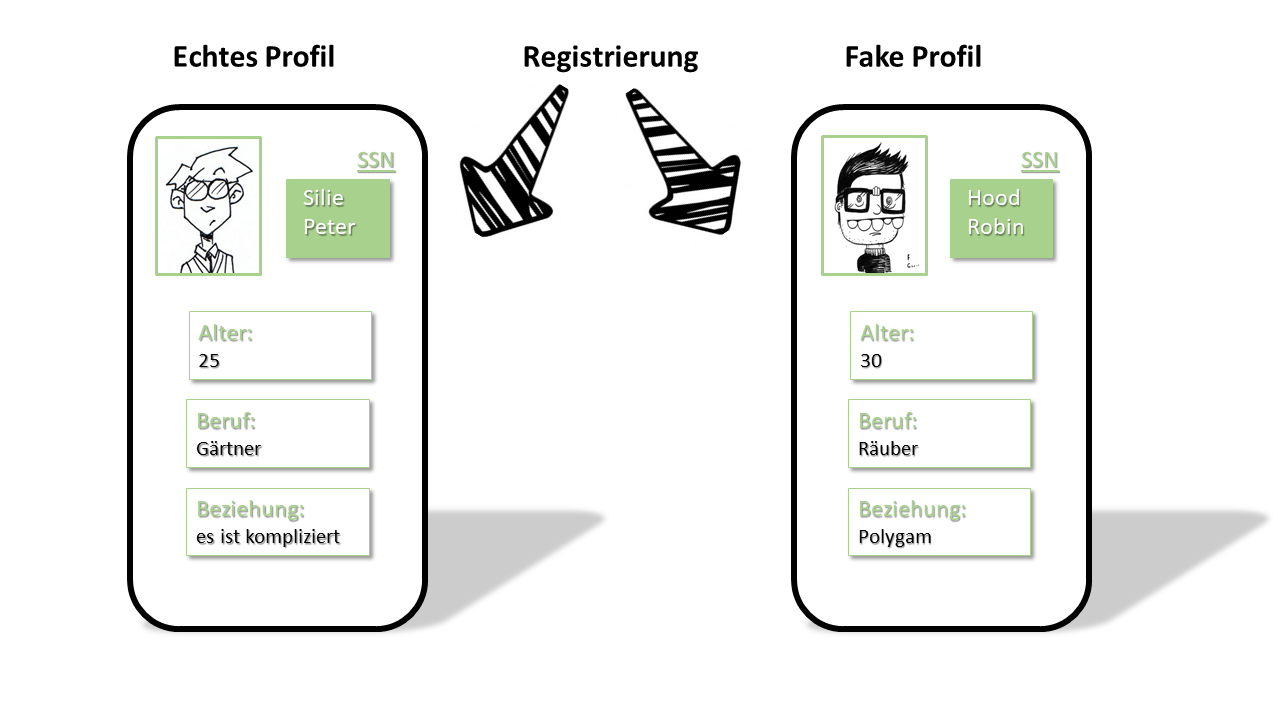
\includegraphics[width=0.8\columnwidth]{figures/Umsetzung1.PNG}
\caption{User legt das Fake-Profil selbst an}
\label{fig:Umsetzung1}
\end{figure}
Ziel dieser Variante ist es, möglichst authentische Fake-Profile zu erstellen. Je authentischer diese auf einen Angreifer wirken, desto sicherer sind die "echten" Daten der Nutzer. \\
In der zweiten Variante erstellt der Nutzer lediglich sein echtes Profil. Er kann jedoch für jede Information, beispielsweise bei seinem Namen, seinem Alter oder seinem Profilbild durch setzen eines Hakens entscheiden, ob diese Information für die Erstellung des Fake-Profils verwendet werden darf, oder nicht. Restliche Daten werden durch das System zufällig generiert. Abbildung \ref{fig:Umsetzung2} veranschaulicht diese Variante. 
\begin{figure}[htbp]
\centering
	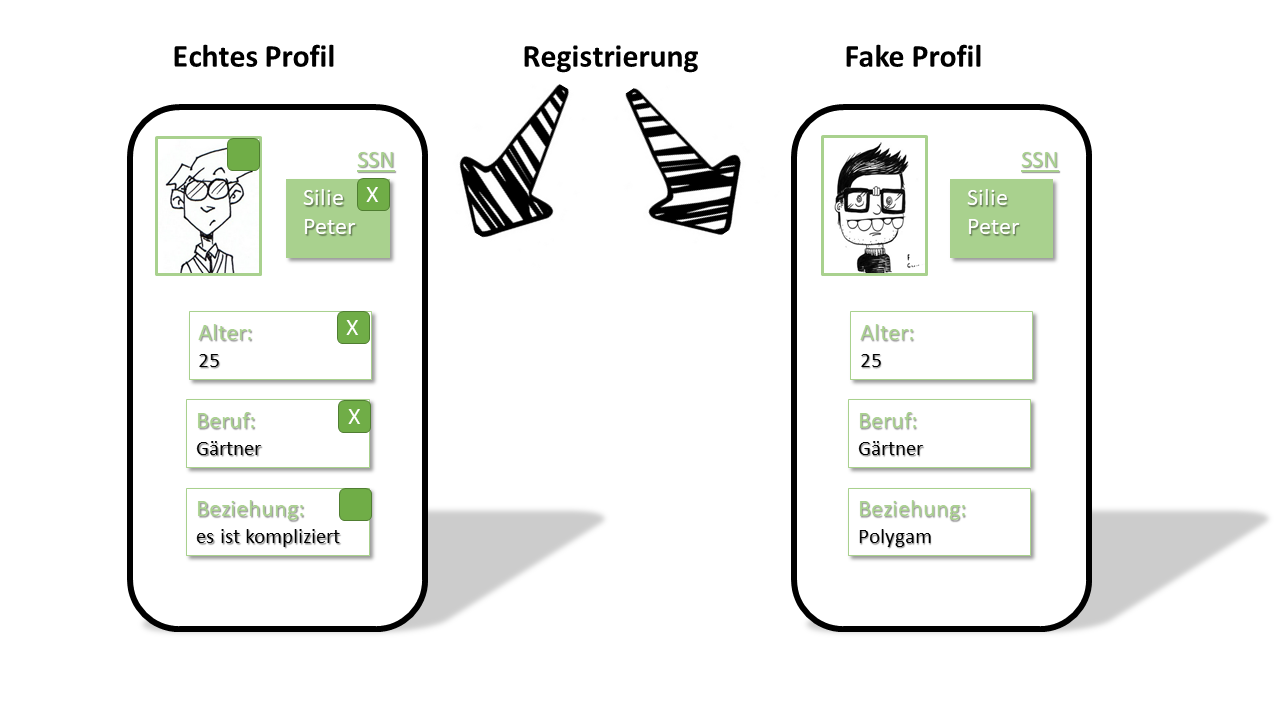
\includegraphics[width=0.8\columnwidth]{figures/Umsetzung2.PNG}
	\caption{Vom User ausgewählte Informationen werden für die Fake-Profile verwendet.}
	\label{fig:Umsetzung2}
\end{figure}
Dadurch sollen durch die Zusatzangaben einerseits authentische Fake-Profile erzeugt werden können und andererseits der zeitliche Aufwand für die Nutzer reduziert werden. \\
In Variante 3 verläuft der gesamte Vorgang automatisiert. Der User hat keinen Einfluss auf die Erstellung der Fake-Profile. Sie werden vom System im Hintergrund generiert. Der Ablauf ist in Abbildung \ref{fig:Umsetzung3} dargestellt.
\begin{figure}[htbp]
\centering
	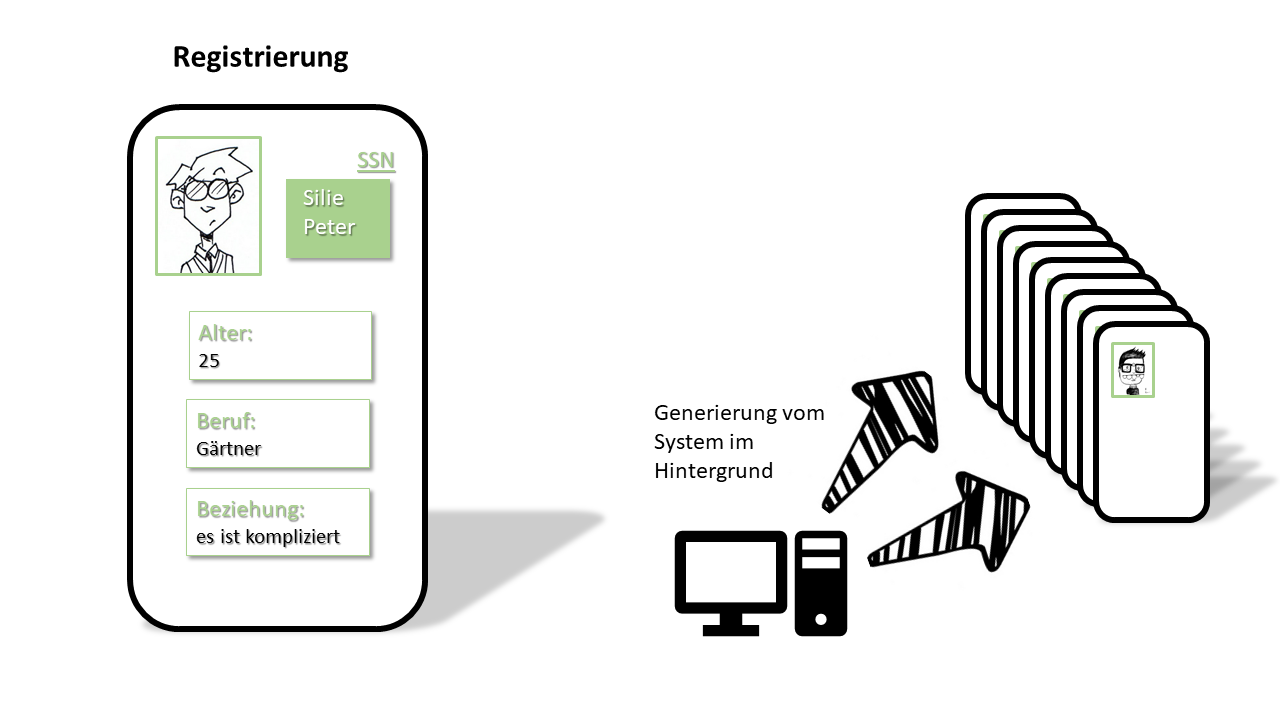
\includegraphics[width=0.8\columnwidth]{figures/Umsetzung3.PNG}
	\caption{Fake-Profile werden vom System generiert.}
	\label{fig:Umsetzung3}
\end{figure}
\\
Variante 4 stellt eine Kombination aus den bisherigen drei Varianten dar. Die Fake-Profile werden, analog zu Variante 3 automatisch generiert. Es besteht jedoch für jeden Nutzer die Möglichkeit Daten, wie beispielsweise Bilder für die Fake-Profil Generierung zur Verfügung zu stellen. Somit ist einerseits kein Nutzer gezwungen Daten bereit zu stellen, andererseits können authentischere Fake-Profile als z.B bei Variante 3 generiert werden. Eine Veranschaulichung dieser Umsetzungsvariante ist am Beispiel von Profilbildern in Abbildung \ref{fig:Umsetzung4} aufgeführt. 
\begin{figure}[htbp]
\centering
	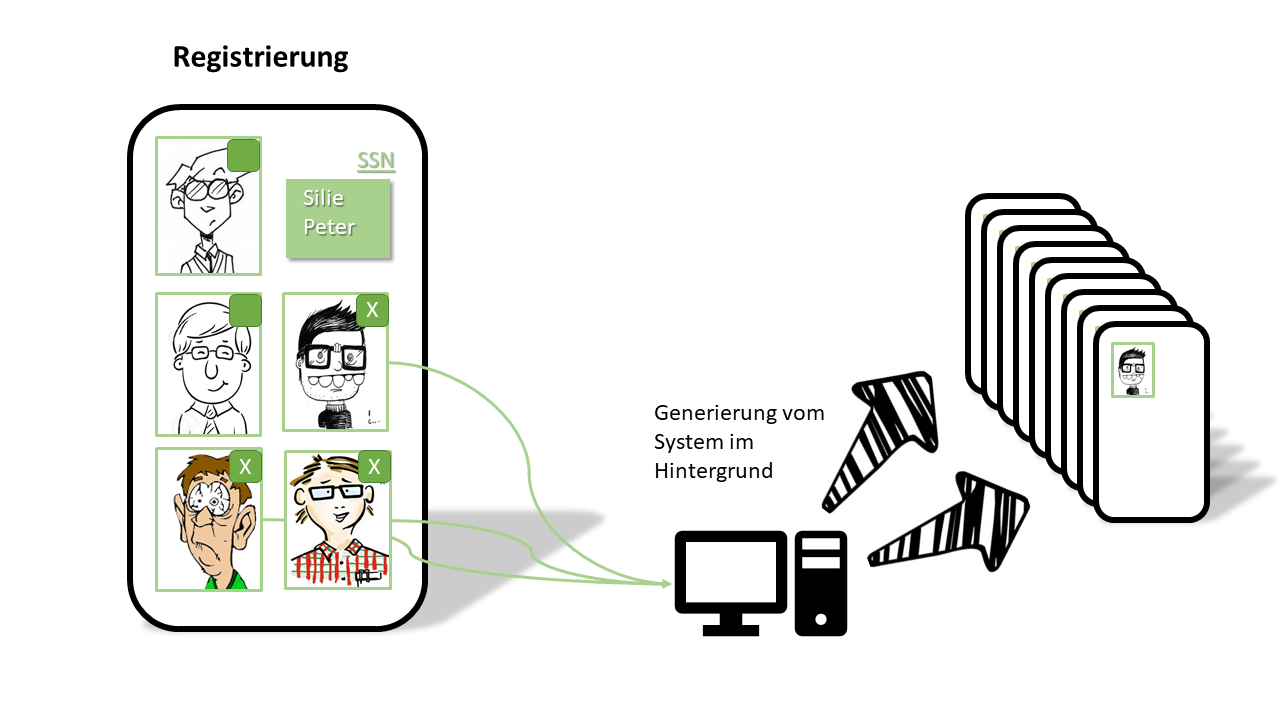
\includegraphics[width=\columnwidth]{figures/Umsetzung4.PNG}
	\caption{Fake-Profile werden vom System generiert. Der User kann freiwillig Daten zur Verfügung stellen.}
	\label{fig:Umsetzung4}
\end{figure}
\section{Methodik}
Für eine Diskussion, welche der Varianten bei Nutzern bevorzugt werden könnte und bei welchen Teilaspekten des Konzepts es möglicherweise Probleme bei der Umsetzung geben könnte, wurde eine Fokusgruppe organisiert. Basierend auf den Ergebnissen der Fokusgruppe wurden interessante Aspekte im Zuge einer Umfrage qualitativ vertieft. Sowohl für die Fokugruppe, als auch für die Umfrage wurden ausschließlich Personen in Betracht gezogen, welche mindestens ein soziales Netzwerk aktiv nutzen. Dadurch soll eine erhöhte Vergleichbarkeit zwischen dem Sicherheitskonzept herkömmlicher Netzwerke und dem im vorherigen Kapitel beschriebenen Konzept erzielt werden. In diesem Kapitel werden zunächst der Aufbau der Fokusgruppe und der Einzelbefragungen erläutert. Anschließend werden die Ergebnisse von beiden zusammengefasst. Basierend darauf erfolgt eine Diskussion potenzieller Herausforderungen bei der Umsetzung des Konzepts. Abschließend werden konkrete Handlungsempfehlungen für die Umsetzung beschrieben.

\subsection{Fokusgruppe}
\label{Fokusgruppe}
Die Fokusgruppe bestand aus dem Projekt Team und 8 Studenten der Hochschule München. Zu Beginn der Fokusgruppe wurden den Teilnehmern allgemeine Fragen zu sozialen Netzwerken gestellt und über potenzielle Schwachstellen bzgl. Sicherheit in vorhandenen Netzwerken diskutiert. Im zweiten Schritt erfolgte die Erläuterung der Konzeptidee und eine anschließende Diskussion bzgl. Machbarkeit, Usability und Sicherheit. Anschließend wurden den Teilnehmern stufenweise alle 4 Umsetzungsvarianten erläutert. Nach jeder Variante erfolgte erneut eine (kurze) Diskussion bezüglich der Machbarkeit, Usability und Sicherheit der jeweiligen Variante. Abschließend erfolgte eine freie Diskussion über die nicht berücksichtigten Aspekte und es wurden weitere Umsetzungsideen erfragt.
 
\subsection{Einzelbefragungen}
\label{Einzelbefragung}
Insbesondere Aspekte, bei denen es mehrere, unterschiedliche Meinungen zwischen den Teilnehmern der Fokusgruppe gegeben hat, wurden im Zuge von Einzelbefragungen vertieft. Hierfür wurden insgesamt 9 Befragungen durchgeführt. Der gesamte Fragebogen ist im Anhang in Abbildung \ref{fig:Fragebogen} angefügt.

\subsection{Ergebnisse}
\label{Ergebnisse}
In Abbildung \ref{fig:MindMap2} ist ein Ausschnitt aus den Ergebnissen der Fokusgruppe und der anschließenden Einzelbefragungen zu sehen. Die gesamten Ergebnisse sind in einem MindMap geclustert im Anhang aufgeführt. Die wichtigsten Aspekte sind im folgenden genauer beschrieben. 
\begin{figure*}[htbp]
	\centering
	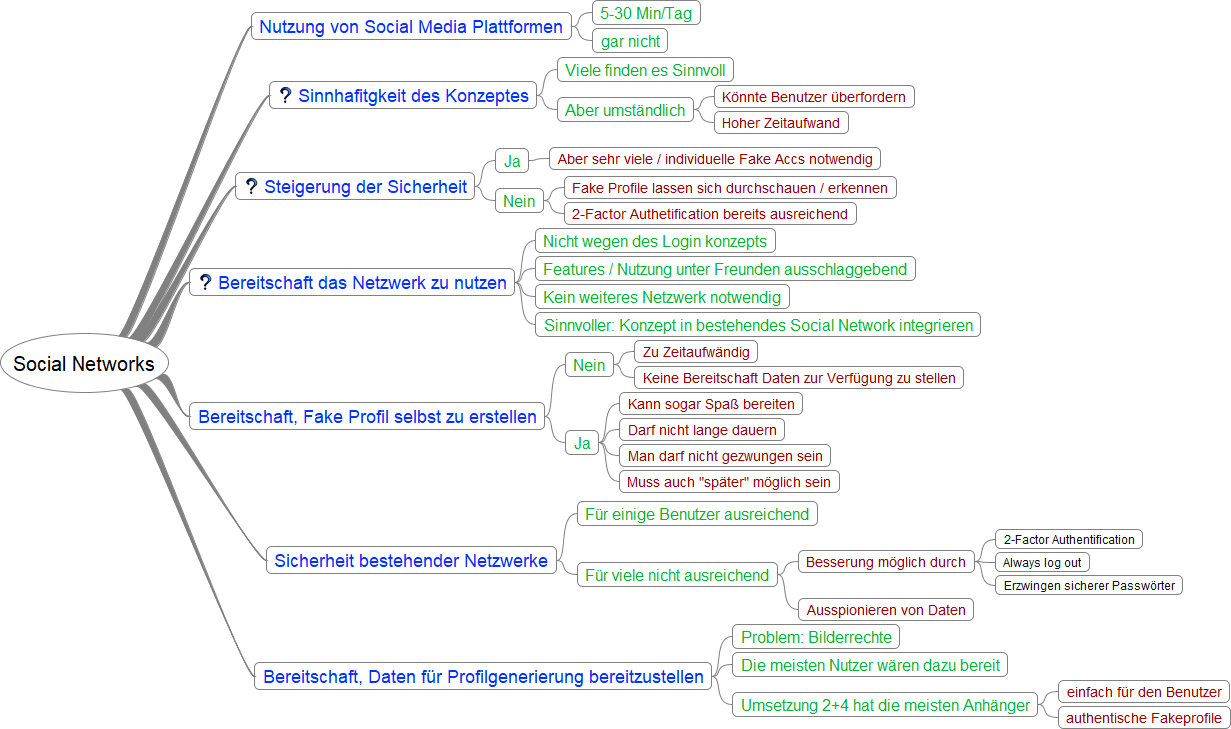
\includegraphics[width=1.5\columnwidth]{figures/Social-Networks_2.png}
	\caption{Ausschnitt aus den Ergebnissen von Fokusgruppe und Einzelbefragung}
	\label{fig:MindMap2}
\end{figure*}
\begin{enumerate}
	\item Für die Usability des Netzwerkes ist es essenziell zu definieren, wann eine Authentifizierung des Nutzers erforderlich ist. Beispielsweise bei wiederholtem Login vom gleichen Gerät sagen die Teilnehmer von Fokusgruppe und Umfrage einstimmig, darf keine erneute Authentifizierung gefordert werden. 
	\item Viele Teilnehmer sehen nicht das Sicherheitskonzept als ausschlaggebend für die Entscheidung, ob sie sich in einem Netzwerk registrieren würden. Andere Aspekte, wie Bekanntheit des Netzwerkes und Anzahl der registrierten Personen, insbesondere der jeweiligen Freunde, wird bei der Wahl eines Netzwerkes als bedeutend wichtiger angesehen.
	\item Der tiefere Sinn dieses Sicherheitskonzeptes ist insbesondere für Personen ohne technische Kenntnisse meist nicht zu verstehen. Folglich wird nur der Mehraufwand bei der Registrierung oder beim Login in das Netzwerk betrachtet. Die Mehrheit der Personen ohne technischen Hintergrund empfanden folglich den Mehraufwand als unnötig. Für die Mehrheit der Personen mit technischem Hintergrund war der Sinn und Zweck des Konzeptes offensichtlich. Diese wären auch mehrheitlich bereit einen gewissen Mehraufwand für eine erhöhte Sicherheit in Kauf zu nehmen. Andererseits beurteilte die Mehrheit der Teilnehmer, unabhängig vom technischen Hintergrund, die Sicherheit bestehender sozialer Netzwerke als nicht ausreichend.
	\item Viele Teilnehmer gaben an, dass sie nicht bereit wären Daten für die Erstellung von Fake-Profilen zur Verfügung zu stellen. Darüber hinaus wären auch nur wenige Teilnehmer bereit Zeit für die Erstellung und Verwaltung von Fake-Profilen zu investieren. Ca. 20\% der Teilnehmer wären weder bereit Daten bereit zu stellen, noch Zeit für die Erstellung der Fake-Profile zu investieren.
	\item Die Mehrheit der Teilnehmer von Fokusgruppe und Umfrage sehen das Zurücksetzen des Logins in das Netzwerk bei Verlust von Login Daten kritisch. Ermöglicht man die Zurücksetzung über eine E-Mail, wird der sicherere Login in das Netzwerk durch eine \glqq einfache\grqq Authentifizierung mittels E-Mail und Passwort ausgehebelt.
	\item Generell sahen die Teilnehmer eine Zwei-Wege Authentifizierung über ein Gerät, in der Regel das Mobiltelefon, als unzureichend. Die Sicherheitsvorkehrungen würde in diesem Fall aufgehoben, sobald ein Angreifer Zugang zum Gerät bekommt.
	\item Insbesondere der Umgang mit den Fake-Profilen führte zu vielen Fragen und Diskussionen. Diese werden im folgenden Kapitel näher erläutert.
\end{enumerate}

\subsection{Diskussion der Herausforderungen bei der Umsetzung des Konzepts}
\label{Diskussion}

Neben den erläuterten Ergebnissen müssen für die Umsetzung des Konzepts auch einige Anmerkungen einzelner Teilnehmer diskutiert werden. In die Diskussion wurden ergänzend auch eigene Lösungsideen und potenziell kritische Punkte eingearbeitet.

\begin{enumerate}
	
	\item Eine große Herausforderung bei der Umsetzung ist die Generierung der Fake-Profile. Einerseits wirken diese authentischer, wenn Mitglieder des Netzwerkes Daten hierfür bereit stellen. Andererseits ist nicht jedes Mitglied bereit Daten bereitzustellen sodass eine Generierung der Fake-Profile ermöglicht werden muss. Darüber hinaus ist es für eine wirkliche Verwirrung des Angreifers durch die sog. "Parallel World" nicht ausreichend, wenn es pro echtes Profil lediglich ein Fake-Profil gibt (statische Generierung bei Registrierung des Teilnehmers). Versucht ein Angreifer beispielsweise das Passwort für ein Konto zu erraten, muss er pro falsches Passwort in einem anderen Fake-Profil landen. Andernfalls kann ein Fake-Profil zu schnell als solches identifiziert werden. Das Sicherheitskonzept funktioniert nur, wenn ein Angreifer keine Möglichkeit hat zwischen einem echten und einem Fake-Profil zu unterscheiden. Es müssen folglich für jedes Profil alle falsch eingegebenen Passwörter (und ggf. weitere Authentifizierungsverfahren wie z.B falsche Codes) gespeichert und mit einem jeweils erstelltem Fake-Profil verknüpft werden (dynamische Generierung bei Bedarf).
	\item Die Lösung der im vorherigen Punkt beschriebenen Herausforderung führt zu einem weiteren Problem. Gerade durch die Vielzahl möglicher Fake-Profile pro echtes Profil, muss eine große Menge Daten gespeichert werden. Dies führt zu einem enormen Bedarf an Speicherkapazität und Rechenleistung, was wiederum einen Anstieg der Kosten für den Betrieb eines solchen Netzwerkes bedeutet. In diesem Zusammenhang wäre ein möglicher Angriffsvektor, dass ein Angreifer versucht das System zu überlasten. 
	\item Es muss ins Detail definiert werden, welche Funktionalitäten den echten und den Fake-Profile zur Verfügung stehen. Eine Kommunikation zwischen Fake-Profilen, sowie zwischen Fake- und echten Profilen muss aus Gründen der Tarnung möglich sein. Dies stellt jedoch eine Gefahr dar, da mittels des Fake-Profils z.B Nachrichten mit Links zu schadhaften Seiten versendet werden können.\\ Andererseits muss sicher gestellt sein, dass jeder Nutzer aus seinem echten Profil auch die echten Profile seiner Kontakte finden kann. Werden aus einem Fake-Profil Nachrichten versendet, müssen diese ebenso wie erstellte oder angezeigte Statusnachrichten oder Bilder im entsprechenden Fake-Profil gespeichert werden. Gelangt man zu einem späteren Zeitpunkt erneut in das Fake-Profil, kann dieses ansonsten enttarnt werden. Es ist jedoch essenziell, dass der Zugriff auf persönliche Daten eines (echten) Profils aus einem Fake-Profil unterbunden wird.
	\item Es ist zu definieren, ob Fake-Profile mittels Suchmaschinen gefunden werden könnte. Beispielsweise kann nahezu jedes Profil im Netzwerk Facebook seit dem Jahr 2007 mittels google gefunden werden \cite{FB_Google}. Findet man jedoch lediglich echte Profile, können Fake-Profile auf diese Weise enttarnt werden. Eine mögliche und umsetzbare Lösung hierfür wäre, wenn jedes Fake-Profil alle öffentliche Informationen eines echten Profils verwendet. Sucht man nun nach dem Profil, ist es ausreichend wenn die öffentlichen Daten des echten Profils angezeigt werden. Da lediglich die öffentlichen Daten sichtbar sind, kann folglich nicht zwischen einem Fake- und einem echten Profil unterschieden werden.
	\item Eine identifizierte Schwachstelle des Netzwerkes sind Personen, die das Mitglied (gut) kennen. Je besser jemand ein Mitglied des Netzwerkes kennt, desto einfacher ist es für diese Person ein potenzielles Fake-Profil dieses Mitglieds zu enttarnen. Grund hierfür ist, dass die Person möglicherweise Freunde, Bekannte oder Familienmitglieder des Mitgliedes kennt. Befindet sich die Person nun in einem potenziellen Fake-Profil in welchem sich keinerlei Nachrichten oder Bilder von besagten Personen befinden, kann dieses als Fake-Profil enttarnt werden. Eine direkte Lösung für diese Problematik konnte nicht identifiziert werden. 
\end{enumerate}

\subsection{Handlungsempfehlungen}
\label{Handlungsempfehlung}
Aus den Ergebnissen der Fokusgruppe, der Einzelbefragungen sowie der diskutierten Aspekte werden nun Handlungsempfehlungen für die Umsetzung des Konzepts herausgearbeitet.

\subsubsection{Speichern des Logins}
Viele Teilnehmer sind nicht bereit viel Zeit in den Authentifizierungsprozess zu investieren. Mechanismen, die es erlauben Logins temporär zu speichern sind Stand der Technik. Diese Mechanismen müssen auch bei diesem Konzept angewendet werden um eine akzeptable Usability zu gewährleisten.

\subsubsection{Integration in ein bestehendes Soziales Netzwerk}
Da Nutzer sich nicht allein wegen dem Sicherheitskonzept in einem Netzwerk registrieren, sondern wegen den bereits registrierten Kontakten, ist es sinnvoll das Konzept in ein bereits bestehendes Netzwerk zu integrieren und kein neues Netzwerk zu entwickeln.
\subsubsection{Klare Erläuterung des Sicherheitskonzeptes}
Durch attraktiv gestaltete Grafiken, Illustrationen, Videos und Anleitungen muss der Benutzer in kurzer Zeit über die Vorteile des Konzepts informiert werden. Auch Personen ohne technische Kenntnisse müssen sowohl den Sinn des Konzeptes verstehen, als auch die Bedienung des Netzwerks beherrschen.
\subsubsection{Automatische und manuelle Fake-Profil Erstellung}
Die Fake-Profil Erstellung muss automatisiert erfolgen. Den Nutzern muss die Möglichkeit gegeben werden Daten für die Generierung des Fake-Profils zur Verfügung zu stellen. Den Nutzern muss bewusst gemacht werden, dass die Fake-Profile durch die Angaben persönlicher (echter) Daten authentischer wirken. Der Mehraufwand für den Nutzer muss jedoch minimiert werden.
\subsubsection{Umgang mit Verlust von Login-Informationen}
Es muss sichergestellt werden, dass auch ein Nutzer, welcher die Login-Informationen verliert, wieder Zugang zu seinem Profil erlangen kann. Zum Beispiel muss das Zurücksetzen des Passworts möglich sein.
\subsubsection{Verfahren für die Zwei-Wege-Authentifizierung}
Dem Nutzer muss eine große Anzahl an hinterlegbaren Authentifizierungsmechanismen zur Auswahl gestellt werden. Zum einen steigert es die Sicherheit, da es für den Angreifer schwerer zu erraten ist, welche Methode die richtige ist. Zum anderen erhöht dies die Usability für den Nutzer, da ihm mehr Auswahlmöglichkeiten zur Verfügung stehen.

\subsubsection{Authentische Fake-Profile}
Die Erstellung von möglichst authentischen Fake-Profilen ist der Kernpunkt des Konzeptes. Sowohl die Kommunikation mit Fake-Profilen, als auch das Suchen von Profilen im Netzwerk muss möglich sein. Fake-Profilen müssen die gleichen Funktionalitäten zur Verfügung stehen, die auch echten Profilen zur Verfügung stehen.

\section{Zusammenfassung und Fazit}
Diese Arbeit beschäftigt sich mit der Umsetzung des Konzeptes aus der Sicht des Nutzers. Zusammenfassend lässt sich sagen, dass zwei wichtige Aspekte für die erfolgreiche Umsetzung dieses Konzeptes zu beachten sind. Zum einen ist eine möglichst einfache Einrichtung und Benutzung des Netzwerks durch den Nutzer essentiell. Dabei sollte der Nutzer möglichst keinen Einfluss den Sicherheitsmechanismus selbst haben. Ihm soll jedoch die Möglichkeit gegeben werden, durch eine freiwillige Bereitstellung von Daten zum Sicherheitskonzept beizutragen. Dadurch soll die Usability sichergestellt und gleichzeitig eine mögliche Fehleinrichtung durch den Nutzer verhindert werden. Die gewohnten Funktionen wie das Verschicken von Nachrichten oder das Teilen von Bildern dürfen durch das neue Konzept nicht eingeschränkt werden. 

Dem gegenüber steht die Generierung von Fake-Profilen. Der Erfolg dieses Konzeptes hängt maßgeblich von der Generierung von möglichst authentischen Profilen ab. Die echte Welt und die Parallelwelt sind keine eigenständigen Konstrukte, sondern müssen mit einander kommunizieren. So können sich zum Beispiel die echten Profile und die dazugehörigen Fake-Profile die öffentlichen Daten teilen. Dabei müssen klare Schnittstellen zwischen echter und Parallelwelt geschaffen werden. Letztendlich lässt sich sagen, dass dieses Konzept in bereits bestehende Netzwerke integriert werden muss. Es hat sich gezeigt, dass Nutzer nicht bereit wären sich nur wegen diesem Sicherheitskonzept in einem Netzwerk zu registrieren. 

\section{Ausblick}
Die Arbeit hat bei der Betrachtung des Konzeptes den Fokus auf den Nutzer gelegt. Es müssen jedoch noch weitere Aspekte für die Umsetzung des Konzepts betrachtet werden. Insbesondere das Angreifermodell muss genauer analysiert werden. Dabei gilt es zu betrachten, ob das Konzept robust gegen bereits bekannte Angriffsszenarien ist. Darüber hinaus ist es notwendig zu untersuchen, ob dieses Konzept neue Angriffsszenarien eröffnet. So könnte ein neues Angriffszenario beispielsweise darin bestehen, durch die mutwillige Erzeugung von zahllosen Fake-Profilen das Netzwerk zu überlasten. 

Viele Fragen stellen sich jedoch erst während der technischen Umsetzung des Konzeptes. Hierfür ist es notwendig einen Prototypen zu erstellen. Die ausgearbeiteten Angriffsmodelle sowie die Usability müssen dann an diesem Prototypen getestet und im Zuge weiterer Studien analysiert und verifiziert werden.

Ein solcher Prototyp kann Probleme bei der Umsetzung aufzeigen und limitierende Faktoren definieren. Darüber hinaus kann dadurch bewertet werden, welche Teilkonzepte am erfolgversprechendsten und welche nicht machbar sind.

%%% END

% BALANCE COLUMNS
\balance{}

% REFERENCES FORMAT
% References must be the same font size as other body text.
\bibliographystyle{SIGCHI-Reference-Format}
\bibliography{sample}

\clearpage
\onecolumn
\section{Anhang}
\begin{figure}[h]
	\centering
	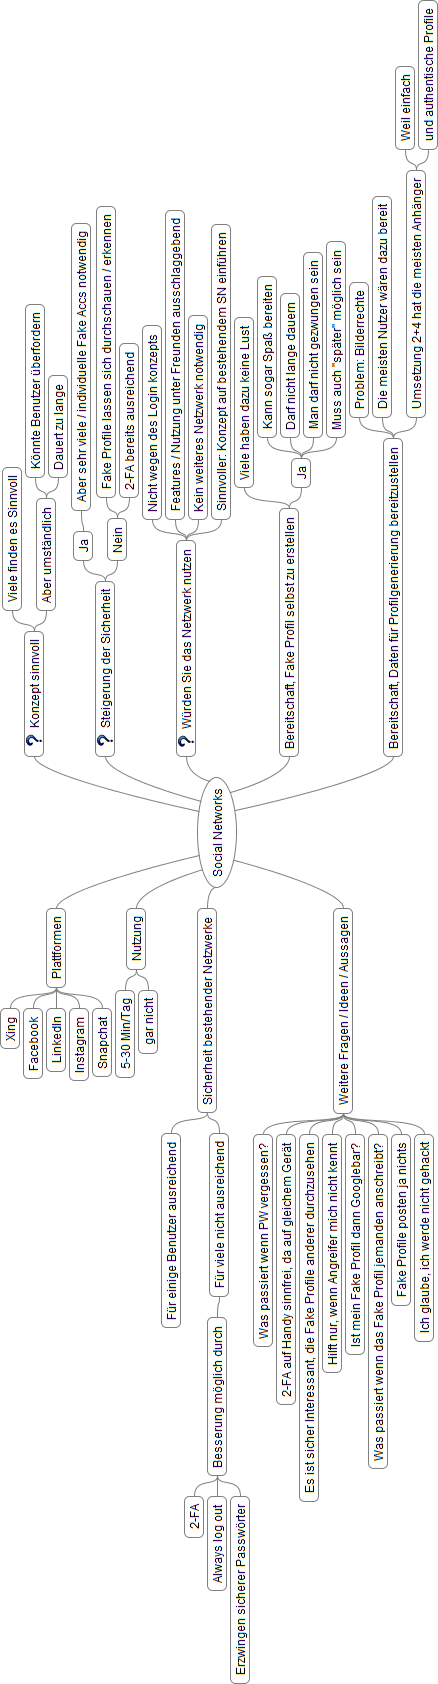
\includegraphics[height=0.76\textheight]{figures/Social-Networks.png}
	\caption{Ergebnisse der Fokusgruppe und der Einzelbefragung}
	\label{fig:MindMapAnhang}
\end{figure}
\newpage
\begin{figure*}[h]
	\centering
	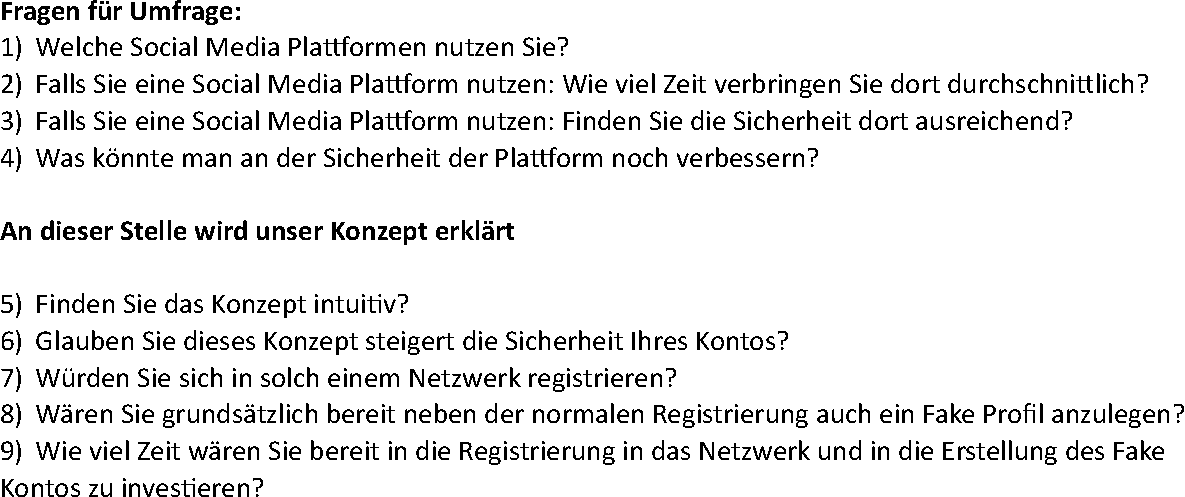
\includegraphics[width=0.8\columnwidth]{figures/Fragebogen.pdf}
	\caption{Aufbau des Fragebogens für die Einzelbefragungen}
	\label{fig:Fragebogen}
\end{figure*}





\end{document}

%%% Local Variables:
%%% mode: latex
%%% TeX-master: t
%%% End:
